\subsection{Data representation}

\begin{frame}{\secname:~\subsecname}

\notesonly{
Each data point $\vec x^{(\alpha)}$ with $\alpha = 1, \ldots, p$ is represented through its relation to all other points in the dataset by measuring pairwise distances.
}

Let $d_{\alpha \alpha^{'}}$ be the pairwise distance between any two points $\vec x^{(\alpha)}$ and $\vec x^{(\alpha')}$. Computing all pairwise distances yields the \emph{distance matrix} $\big\{ d_{\alpha \alpha^{'}} \big\}$:

\begin{equation}
\label{eq:pairwisedistdef}
d: \mathbb{R}^N \times \mathbb{R}^N 
    \rightarrow \mathbb{R}_0^+ \quad\text{ i.e.}\;\; d \ge 0
\end{equation}

The components of the distance matrix are subject to the following constraints:
\begin{itemize}
\item The distance of a point to itself is zero.
\item The distance matrix is symmetric.
\end{itemize}

\end{frame}
\begin{frame}\frametitle{Choice of distance measure}

A simple and common choice of measure is squared Euclidean distance:

\begin{equation}
\label{eq:pairwisedisteuclidean}
d_{\alpha \alpha^{'}} := \frac{1}{2} \big(
    \vec{x}^{(\alpha)} - \vec{x}^{(\alpha^{'})} \big)^2
\end{equation}

\notesonly{
Another possibility for populating the components of the distance matrix is to base this high-dimensional relation of one point to another on \emph{scalar product}, the ``kernel trick''\footnote{As encountered in Kernel-PCA}. 
The distance is measured for a pair of points in some high-dimensional space $\phi$
}
\slidesonly{
Or elements derived via a ``kernel trick'':
}

$$
          \vec{\phi}: \vec{x}^{(\alpha)} \rightarrow
          \vec{\phi}_{\big( \vec{x}^{(\alpha)} \big)}
          \equiv \vec{\phi}^{(\alpha)}
$$

\begin{align}
			d_{\alpha \alpha^{'}} 
			& = \frac{1}{2} \big( \vec{\phi}^{(\alpha)} 
				- \vec{\phi}^{(\alpha^{'})} \big)^2 \\
			& = \frac{1}{2} \Big\{ \big( \vec{\phi}^{(\alpha)}
				\big)^2 - 2\big( \vec{\phi}^{(\alpha)} \big)^\top
				\vec{\phi}^{(\alpha^{'})} + \big(
				\vec{\phi}^{(\alpha^{'})} \big)^2 \Big\} \\
			& = \frac{1}{2} \bigg\{ k_{\big( \vec{x}^{(\alpha)},
				\vec{x}^{(\alpha)} \big)} 
				- 2k_{\big(\vec{x}^{(\alpha)},
				\vec{x}^{(\alpha^{'})} \big)}
				+ k_{\big(\vec{x}^{(\alpha^{'})},
				\vec{x}^{(\alpha^{'})} \big)}
				\bigg\}
\end{align}

\end{frame}

\begin{frame}
\slidesonly{\frametitle{Other sources for pairwise distances}}

A further use-case is one where pairwise distance is not measured explicitly. The data representation can already be in a pairwise fashion as a result of an algorithm.\\
Example: Sequence alignment procedures and graph-similarity measures produce pairwise representations.\\

We will opt for the \emph{squared Euclidean distance} for our pairwise clustering algorithm.

\end{frame}

\begin{frame}{Possibilities: transformed distances}

\begin{center}
\begin{minipage}{0.99\textwidth}
	\begin{center}
	\begin{minipage}{0.35\textwidth}
		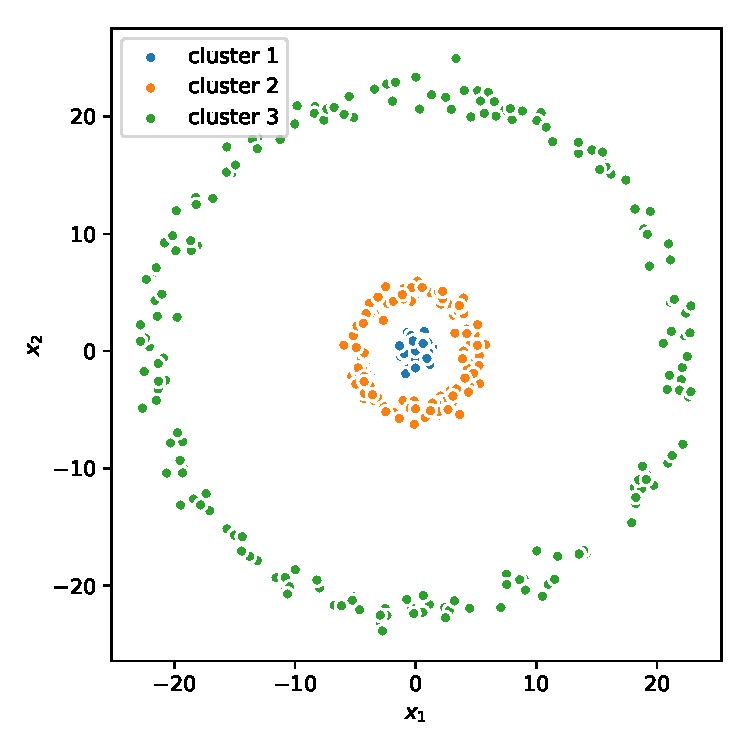
\includegraphics[width=0.9\textwidth]{img/m3_circ_data} 
	\end{minipage}
	\begin{minipage}{0.35\textwidth}
		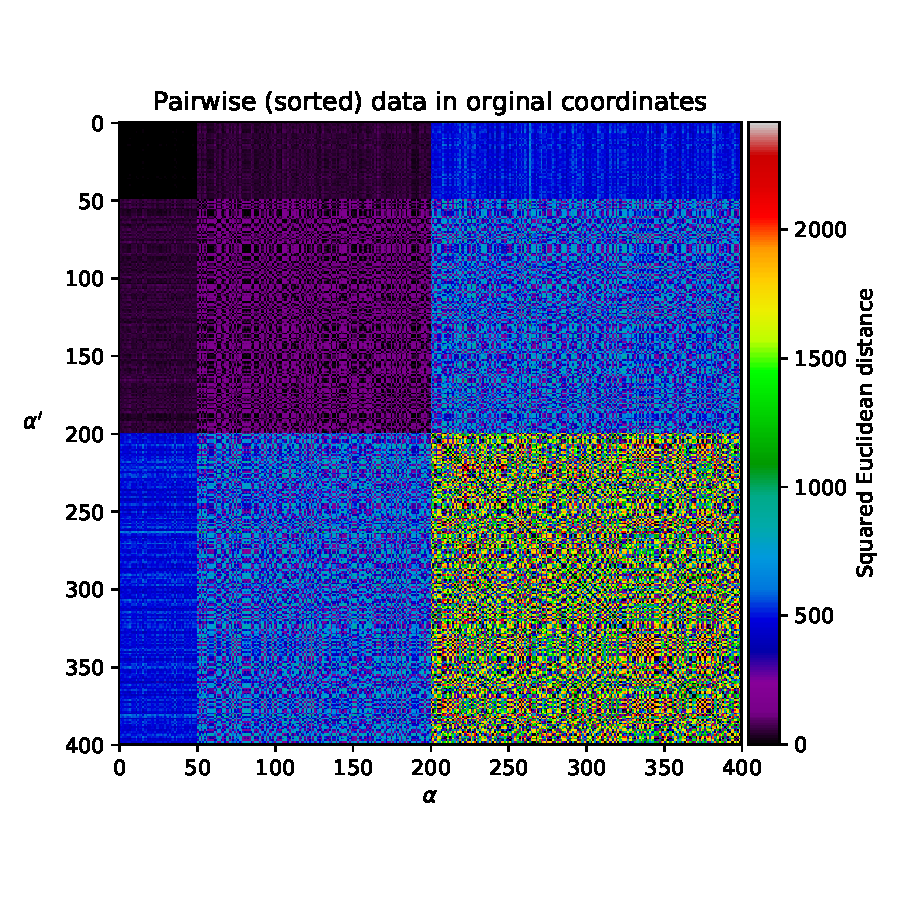
\includegraphics[width=0.9\textwidth]{img/m3_circ_pdist} 
	\end{minipage}
	\end{center}
\end{minipage}
\end{center}

\begin{center}
\begin{minipage}{0.99\textwidth}
	\begin{center}
	\begin{minipage}{0.35\textwidth}
		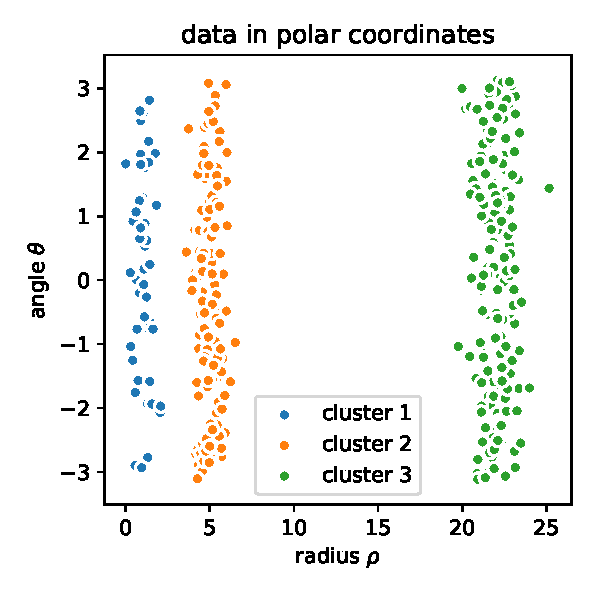
\includegraphics[width=0.9\textwidth]{img/m3_circ_data_polar} 
	\end{minipage}
	\begin{minipage}{0.35\textwidth}
		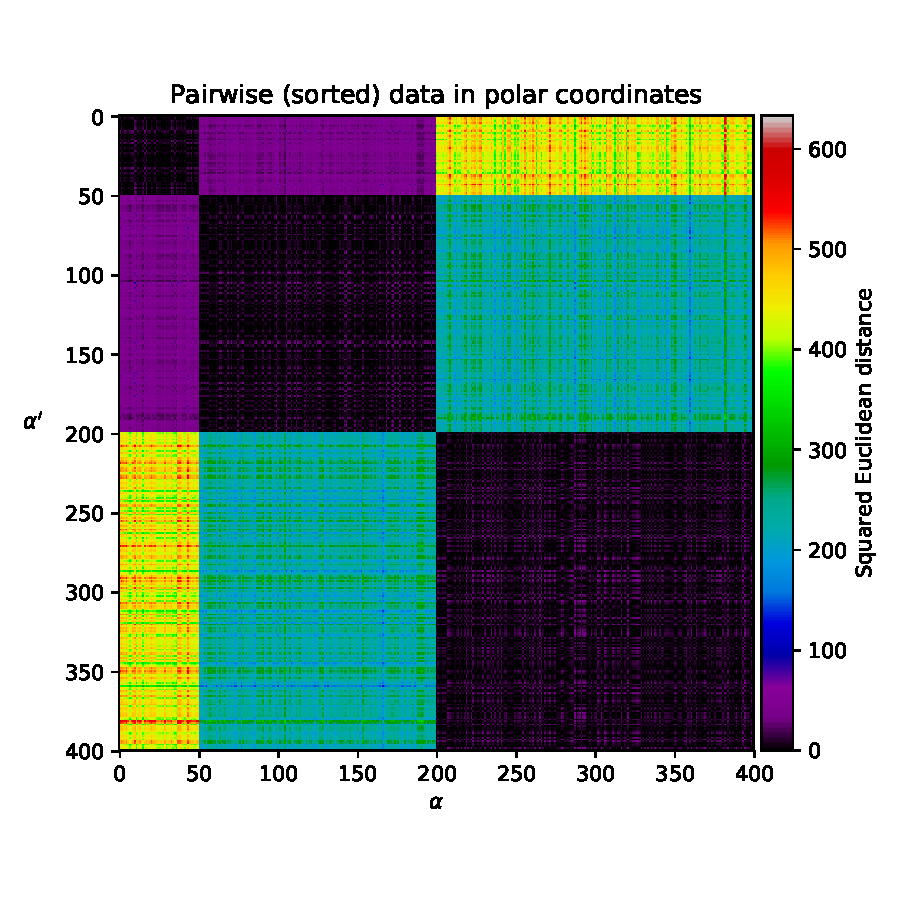
\includegraphics[width=0.9\textwidth]{img/m3_circ_pdist_polar} 
	\end{minipage}
	\end{center}
\end{minipage}
\end{center}

\end{frame}

\subsection{Cost}

\begin{frame}
\frametitle{Pairwise Clustering: Problem statement}

\begin{itemize}
\itr set of clusters (partitions): $q = 1, \ldots, M$
\itr observations (feature vectors): $\vec{x}^{(\alpha)}, \; 
\alpha = 1, \ldots, p; \; \vec{x}^{(\alpha)} = \mathbb{R}^N$
\itr binary assignment variable:
$$ m_q^{(\alpha)} := \left\{ \begin{array}{ll}
		1, & \text{if object } \alpha \text{ belongs to cluster } q \\\\
		0, & \text{otherwise}
	\end{array} \right.
$$
\itr distance matrix $d_{\alpha \alpha^{'}}$ populated using squared Euclidean distance:
$$
	d_{\alpha \alpha^{'}} := \frac{1}{2} \big( \vec{x}^{(\alpha)} 
		- \vec{x}^{(\alpha^{'})} \big)^2
$$
\end{itemize}
\end{frame}
\begin{frame}
\frametitle{Cost function \& model selection}
\begin{align}
E_{ \big[ \big\{ m_q^{(\alpha)} \big\} \big] }
	&= \frac{1}{2p} \sum\limits_q \sum\limits_{\alpha}
	 \overbrace{ \frac{\sum\limits_{\alpha^{'}} 
		m_q^{(\alpha)}m_q^{(\alpha^{'})} d_{\alpha \alpha^{'}}}{
                \sum\limits_{\alpha'} m_q^{(\alpha')}
		}}^{ \substack{	\text{avg. distance between} \\
				\alpha \text{ and \textbf{all other} objects $\alpha'$} \\
				\text{from the \textbf{same} cluster } q}}\\
&= \frac{1}{2p} \sum\limits_q \frac{ \sum\limits_{\alpha \alpha^{'}}
		m_q^{(\alpha)} m_q^{(\alpha^{'})} \big( \vec{x}^{(\alpha)}
		-\vec{x}^{(\alpha^{'})} \big)^2 }{
			\sum\limits_{\alpha} m_q^{(\alpha)}}
	\eqexcl \min_{\big\{ m_q^{(\alpha)} \big\}}
\end{align}
            
\end{frame}

\subsection{Relation of pairwise clustering to K-means}

\begin{frame}\frametitle{\subsecname}

\notesonly{
When we choose squared Euclidean distance as the distance measure for pairwise clustering, we can show that this choice lets pairwise clustering effectively find the same solution as K-means clustering.
}

\begin{center}
\resizebox{.7\textwidth}{!}{%
\begin{tabular}{cllll}
Pairwise Clustering                                                                 & \multicolumn{1}{c}{$\Longrightarrow$} & \multicolumn{1}{c}{\begin{tabular}[c]{@{}c@{}}Some\\ clustering solution\end{tabular}} & \multicolumn{1}{c}{$\Longleftarrow$} & K-means \\
\begin{tabular}[c]{@{}c@{}}using\\ $d_{\alpha\alpha'}$ := sq. Eucl. distance\end{tabular} &                                     &                                                                                        &                                  &       
\end{tabular}%
}
\end{center}

\end{frame}

\begin{frame}\slidesonly{\frametitle{Relation of pairwise clustering to K-means}}

\begin{equation}
	\begin{array}{ll}
	E_{\big[ \big\{ m_q^{(\alpha)} \big\} \big]}
\only<1> {
	& = \frac{1}{2p} \sum\limits_q \frac{ \sum\limits_{\alpha \alpha^{'}}
		m_q^{(\alpha)} m_q^{(\alpha^{'})} \big( \vec{x}^{(\alpha)}
		-\vec{x}^{(\alpha^{'})} \big)^2 }{
			\sum\limits_{\alpha} m_q^{(\alpha)}} \\\\
	& = \frac{1}{2p} \sum\limits_q \frac{ 
		\sum\limits_{\alpha} \sum\limits_{\alpha^{'}}
		m_q^{(\alpha)} m_q^{(\alpha^{'})} \Big\{ \big( 
		\vec{x}^{(\alpha)} \big)^2 - 2\big( \vec{x}^{(\alpha)} \big)^\top
		\vec{x}^{(\alpha^{'})} + \big( \vec{x}^{(\alpha^{'})} \big)^2
		\Big\}
		}
		{ \sum\limits_{\alpha} m_q^{(\alpha)} } \\\\
}
\only<1,2> {
	& = \frac{1}{2p} \sum\limits_q \Bigg\{
		\frac{ 
		\sum\limits_{\alpha} {\color{blue}\sum\limits_{\alpha^{'}}}
		m_q^{(\alpha)} {\color{blue}m_q^{(\alpha^{'})} }
		\big( \vec{x}^{(\alpha)} \big)^2 }
		{ \color{red}\sum\limits_{\alpha}  {m_q^{(\alpha)}}
		} \\
		&\qquad- 2
		\frac{ \sum\limits_{\alpha} \sum\limits_{\alpha^{'}}
		m_q^{(\alpha)} m_q^{(\alpha^{'})} 
		\big( \vec{x}^{(\alpha)} \big)^\top
		\vec{x}^{(\alpha^{'})} }
		{ \sum\limits_{\alpha} m_q^{(\alpha)} } 
		+ 
		\frac{ {\color{red}\sum\limits_{\alpha}} \sum\limits_{\alpha^{'}}
		{\color{red}m_q^{(\alpha)}}m_q^{(\alpha^{'})} 
		\big( \vec{x}^{(\alpha^{'})} \big)^2
		}
		{\color{red}\sum\limits_{\alpha} m_q^{(\alpha)} } \Bigg\}
		\\
}
	\pause
\only<2> {
		&
		{\scriptscriptstyle
		\text{with} \;
			{\color{red}\sum\limits_{\alpha} m_q^{(\alpha)}} = {\color{blue}\sum\limits_{\alpha'} m_q^{(\alpha')}}
		\; \text{follows:}
		}
		\\
	& = \frac{1}{2p} \sum\limits_q \Bigg\{
		\frac{ 
		\sum\limits_{\alpha}
		m_q^{(\alpha)} 
		\big( \vec{x}^{(\alpha)} \big)^2 {\color{blue}\sum\limits_{\alpha^{'}} m_q^{(\alpha^{'})}} }
		{ \color{blue} \sum\limits_{\alpha^{'}} m_q^{(\alpha^{'})} } \\
		&\qquad - 2
		\frac{ \sum\limits_{\alpha} \sum\limits_{\alpha^{'}}
		m_q^{(\alpha)} m_q^{(\alpha^{'})} 
		\big( \vec{x}^{(\alpha)} \big)^\top
		\vec{x}^{(\alpha^{'})} }
		{ \sum\limits_{\alpha^{'}} m_q^{(\alpha^{'})} }
		 + 
		\frac{ \sum\limits_{\alpha} m_q^{(\alpha)^{'}}
		\big( \vec{x}^{(\alpha^{'})} \big)^2 {\color{red}\sum\limits_{\alpha} m_q^{(\alpha)}}
		}
		{ \color{red}\sum\limits_{\alpha} m_q^{(\alpha)} } \Bigg\}
		\\\\
}
	\pause
\only<3> {
	& = \frac{1}{2p} \sum\limits_q \Bigg\{
		{ 
		\sum\limits_{\alpha}
		m_q^{(\alpha)} 
		\big( \vec{x}^{(\alpha)} \big)^2 }
		\\
		&\quad  
		- 2 \Big( \sum\limits_{\alpha} m_q^{(\alpha)} \big( 
		\vec{x}^{(\alpha)} \big)^\top \Big) 
		\underbrace{ \frac{ \sum\limits_{\alpha^{'}} m_q^{(\alpha^{'})} 
		\vec{x}^{(\alpha^{'})} }{ \sum\limits_{\alpha^{'}} 
		m_q^{(\alpha^{'})} } }_{
			\substack{ \eqexcl \vec{w}_q \\
				\substack{\text{centroid =} \\ 
                                  \text{center of mass}\\ 
                                  %\text{ ({\it cf. \ref{kmeans_modelselection}})}
                                  } 
                                  }
                                  }
		+
		{ \sum\limits_{\alpha^{'}} m_q^{(\alpha^{'})}
		\big( \vec{x}^{(\alpha^{'})} \big)^2 }
		\Bigg\}
		\\
		&{\scriptscriptstyle
		\text{with} 
			\; { \sum\limits_{\alpha} m_q^{(\alpha)}
			\big( \vec{x}^{(\alpha)} \big)^2 }
			= { \sum\limits_{\alpha^{'}} m_q^{(\alpha^{'})}
			\big( \vec{x}^{(\alpha^{'})} \big)^2 } 
		\; \text{follows:}
		}
		\\
	& = \frac{1}{2p} \sum\limits_q \Big\{
		2\, \sum\limits_{\alpha}
		m_q^{(\alpha)} 
		\big( \vec{x}^{(\alpha)} \big)^2
		- 2 
		\Big( 
			\sum\limits_{\alpha} m_q^{(\alpha)} \big( 
			\vec{x}^{(\alpha)} \big)^\top 
		\Big) \,
		\vec{w}_q
		\Big\} \\\\
}
\pause
\only<4>{
	& = \frac{1}{p} \sum\limits_{q, \alpha} m_q^{(\alpha)} \Big\{
		\big( \vec{x}^{(\alpha)} \big)^2 - \big( \vec{x}^{(\alpha)}
		\big)^\top \vec{w}_q \Big\} \\\\
	& = \frac{1}{p} \sum\limits_{q, \alpha} m_q^{(\alpha)} \Big\{
		\big( \vec{x}^{(\alpha)} \big)^2 - \big( \vec{x}^{(\alpha)}
		\big)^\top \vec{w}_q - \vec{w}_q^2
		+ \vec{w}_q^2 \Big\} \\
		
		
		&{\scriptscriptstyle\text{with} \; 
			\vec w_q^2 = \vec w_q^\top \vec w_q = \frac{ \sum\limits_{\alpha} m_q^{(\alpha)} \big(
					\vec{x}^{(\alpha)} \big)^\top }{
						\sum\limits_{\alpha} m_q^{(\alpha)}}
				\cdot \vec{w}_q \;
		\; \text{follows:}
		}
		\\
	& = \frac{1}{p} \sum\limits_{q, \alpha} m_q^{(\alpha)} \Big\{ 
		\big( \vec{x}^{(\alpha)} \big)^2 - 2 \big( \vec{x}^{(\alpha)}
		\big)^\top \vec{w}_q + \vec{w}_q^2 \Big\} \\\\
	& = \frac{1}{p} \sum\limits_{q, \alpha} m_q^{(\alpha)} \big( 
		\vec{x}^{(\alpha)} - \vec{w}_q \big)^2 \\\\
	& = E_{\big[ \big\{ m_q^{(\alpha)} \big\}, \big\{ \vec{w}_q \big\} \big]} 
 \corresponds \text{ cost function for K-Means}
 }
	\end{array}
\end{equation}
\end{frame}

\begin{frame}{\subsecname}

\slidesonly{
\begin{center}
	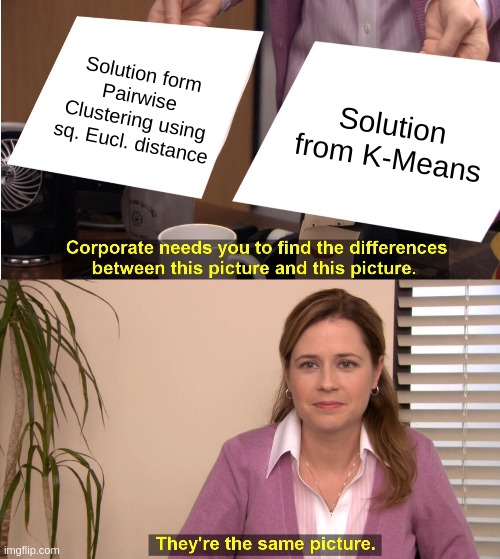
\includegraphics[width=0.4\textwidth]{img/meme_pariwseeuclkmeans}
\end{center}
}

\notesonly{
We've seen that Pairwise Clustering based on squared Euclidean distance boils down to K-means. Pairwise clustering can therefore be considered a generalization of K-means. One can also think of K-means as a special case of pairwise clustering.}
\slidesonly{
K-means is a special case of pairwise clustering.
}

\end{frame}

\begin{frame}{Pairwise clustering: A discrete optimization problem}

Recall that the assignment variables are defined as binary to reflect hard assignments. Therefore, the optimization problem for pairwise clustering in the general case is a \emph{discrete optimization problem}.

\notesonly{
The consequence of this is that gradient-based methods are no longer applicable and that rather methods of combinatorial optimization are needed. We've encountered two variants for such:
}

\begin{itemize}
\item simulated (stochastic) annealing. Fairly simple, robust to local minima but slow.
\item mean-field (deterministic) annealing. An effective approximation for stochastic optimization which can be computed much faster.
\end{itemize}

\end{frame}
\begin{frame}

Recall from mean-field annealing:
\notesonly{
The individual state variables $s_k$ in the state vector $\vec s$ were assumed to be \emph{independent}. This implies the factorization of their moments under the approximated distribution $Q$ (i.e. 
\begin{equation}
\label{eq:factorizingmoments}
\implies
    \langle \Pi_k s_k \rangle_Q = \Pi_k \langle s_k\rangle_Q.
\end{equation}
When we use mean-field annealing in the context of pairwise clustering, it is the assignment variables $m_q^{(\alpha)}$ that stand for the state variables. The assignment is based on \textbf{pairwise} distance, this violates our assumption of having independent state variables. $m_q^{(\alpha)}$ is not completely independent of $m_q^{(\alpha')}$.
 Therefore, the 
calculation of moments and mean-fields must be adapted.
}
\slidesonly{
\begin{itemize}
\item $s_k$ in the state vector $\vec s$ were assumed to be \emph{independent}
\item $\implies
    \langle \Pi_k s_k \rangle_Q = \Pi_k \langle s_k\rangle_Q
    \quad \!\! (\substack{\text{moments}  \\ \text{factorize}})$
\item mean-field annealing in the context of pairwise clustering: $m_q^{(\alpha)}$ for state variables
\item \textbf{but} $m_q^{(\alpha)}$ is \textbf{not} completely independent of $m_q^{(\alpha')}$
\end{itemize}
}

\end{frame}

